\subsection{Độ đo}
Trong bài toán nhận dạng người đi bộ (pedestrian detection), nhóm đã sử dụng một độ đo phổ biến trong thị giác máy tính là mean Average Precision (mAP) cho việc đánh giá hiệu suất của hai phương pháp HOG+SVM và Faster R-CNN. Độ đo này được sử dụng để đánh giá độ chính xác của việc phát hiện và định vị vị trí của các người đi bộ trong hình ảnh. mAP được đo trong khoảng từ 0 đến 1.

\subsubsection{IOU}
IOU (Intersection over Union) là một phép đo sử dụng để đánh giá sự chồng chéo giữa hai khu vực được dự đoán và khu vực thực tế trong bài toán nhận dạng đối tượng. Trong bước tính mAP (mean Average Precision), IOU được sử dụng để xác định xem một đối tượng dự đoán được coi là chính xác hay không.

Để tính toán IOU, ta sử dụng hai khu vực là khu vực dự đoán (predicted region) và khu vực thực tế (ground truth region). Khu vực này được biểu diễn bằng các hình chữ nhật hoặc các đa giác đối tượng trong không gian 2D.

IOU được tính bằng cách tính tỷ lệ diện tích của khu vực giao nhau (intersection) giữa hai khu vực và diện tích của khu vực hợp nhau (union) giữa hai khu vực. Công thức tính toán IOU:
%nói về iou trước
\graphicspath{{figures/}}
\begin{figure}[h!]
  \centering
  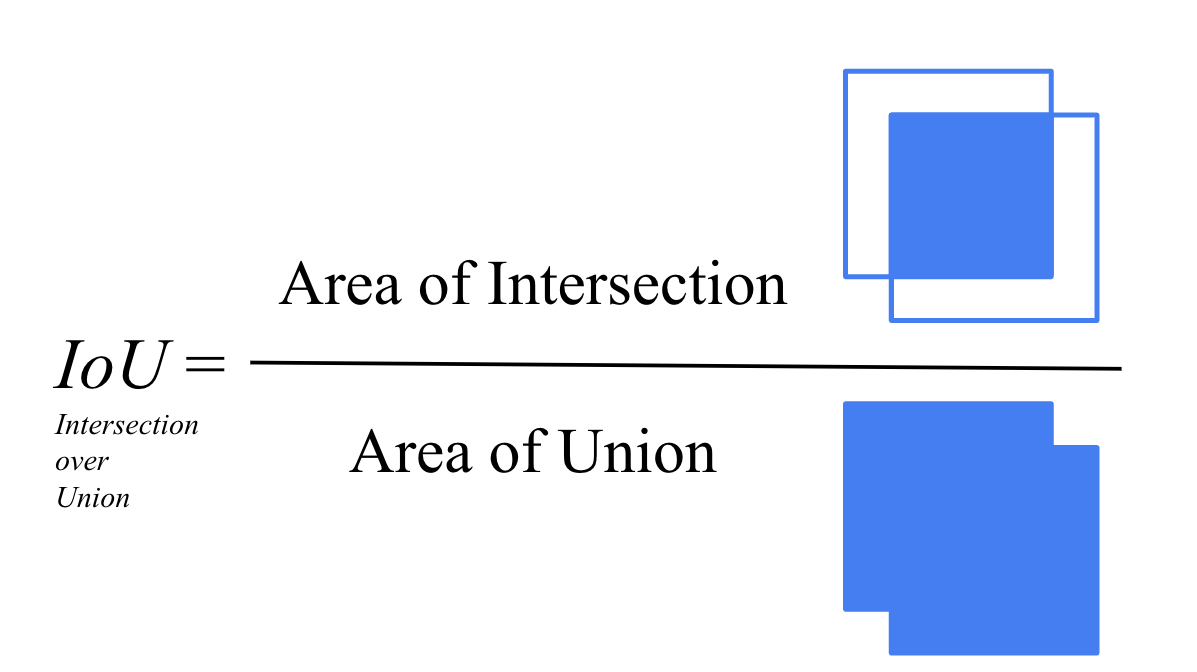
\includegraphics[scale=0.24]{graphics/iou.png}
  \caption{Cách tính IoU}
\end{figure}

Giá trị IOU nằm trong khoảng từ 0 đến 1. Nếu IOU = 0, tức là không có sự chồng chéo giữa khu vực dự đoán và khu vực thực tế. Ngược lại, nếu IOU = 1, tức là khu vực dự đoán trùng khớp hoàn toàn với khu vực thực tế.

Trong bước tính toán mAP, mỗi đối tượng dự đoán được so sánh với các đối tượng thực tế. Nếu IOU của đối tượng dự đoán với đối tượng thực tế vượt qua một ngưỡng xác định (thường là 0.5), đối tượng dự đoán được coi là chính xác. Ngược lại, nếu IOU không đạt ngưỡng này, đối tượng dự đoán được coi là sai.

\subsubsection{Confusion Matrix}
Ứng với mỗi ngưỡng xác định (IOU threshold), ta được một cặp giá trị precision và recall. Sau khi tính IOU và căn cứ vào ngưỡng xác định, ta sử dụng confusion matrix để phân tích và phân nhóm các trường hợp dự đoán của mô hình. Thông qua confusion matrix, ta có thể phân loại các trường hợp như Hình \ref{fig:confusion-matrix}.
\graphicspath{{figures/}}
\begin{figure}[h!]
  \centering
    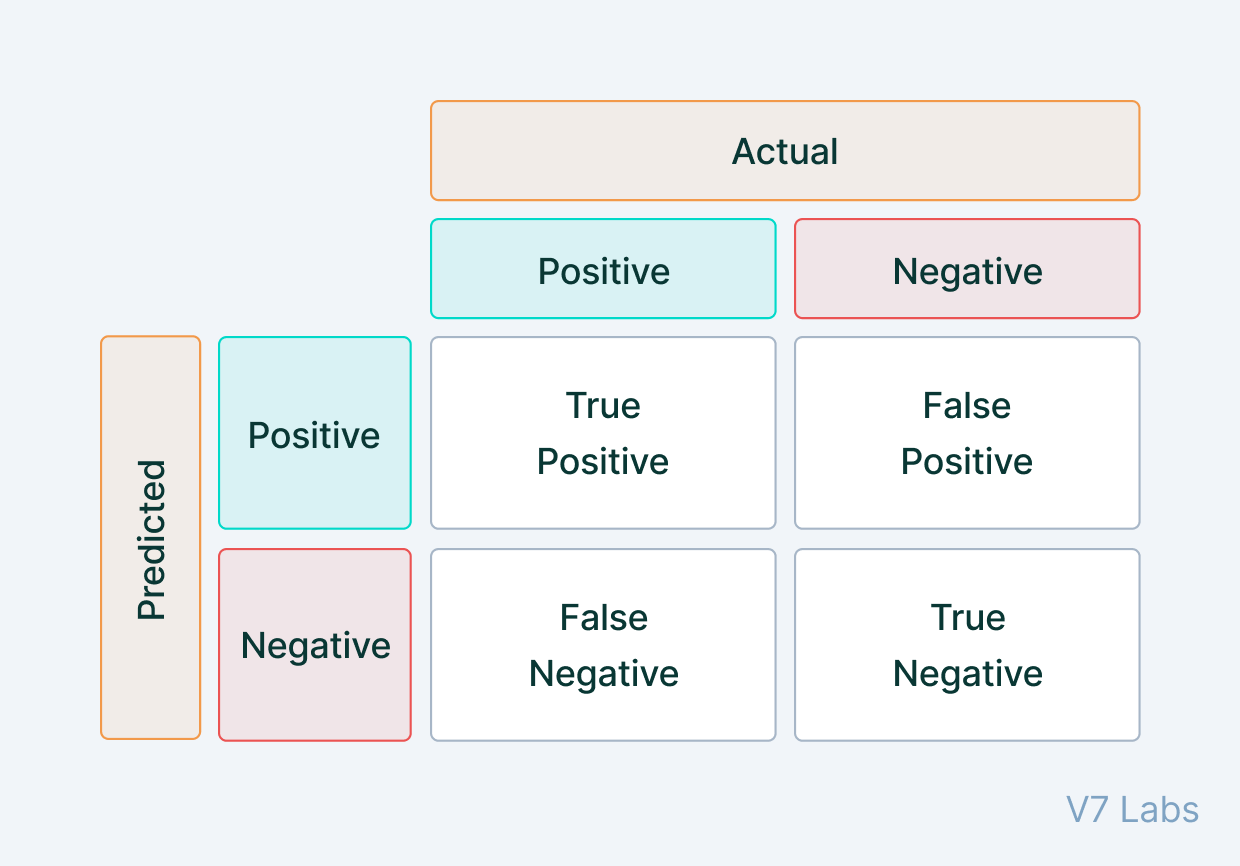
\includegraphics[scale=0.5]{graphics/confusion-matrix.png}
  \caption{Confusion matrix}
  \label{fig:confusion-matrix}
\end{figure}

\subsubsection{Tính toán mAP}
Mean Average Precision (mAP) là một độ đo tổng hợp của các giá trị Average Precision (AP) tính toán cho từng lớp (trong trường hợp này, lớp người đi bộ) trong bộ dữ liệu. Để tính toán AP, ta xây dựng đường cong Precision-Recall bằng cách thay đổi ngưỡng (threshold) phân loại và tính toán precision và recall tại mỗi ngưỡng.

Precision là tỷ lệ giữa số lượng các đối tượng được phát hiện chính xác và tổng số đối tượng được phát hiện
\begin{equation*}
    Precision = \frac{TP}{TP + FP}\nonumber
\end{equation*}
Trong khi Recall là tỷ lệ giữa số lượng các đối tượng được phát hiện chính xác và tổng số đối tượng thực tế trong hình ảnh.
\begin{equation}
    Recall = \frac{TP}{TP + FN}\nonumber
\end{equation}

Sau khi tính toán được đường cong Precision-Recall, ta tính toán giá trị AP bằng cách tính toán diện tích dưới đường cong Precision-Recall. Giá trị AP đại diện cho độ chính xác trung bình của việc phát hiện đối tượng trong các ngưỡng phân loại khác nhau. Mean Average Precision (mAP) là giá trị trung bình của AP cho tất cả các lớp (ở bài toán pedestrian detection là 1).
\begin{equation}
    mAP = \frac{|TP|}{|TP| + |FP|}\nonumber
\end{equation}
\begin{figure}[h!]
  \centering
    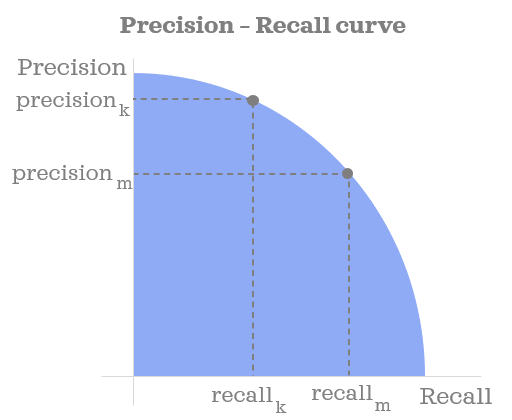
\includegraphics[scale=0.5]{graphics/curve.png}
  \caption{Đường cong Precision-Recall}
\end{figure}
Một giá trị mAP cao cho thấy hai phương pháp đều đạt được độ chính xác cao trong việc phát hiện người đi bộ trong hình ảnh. Tuy nhiên, cần lưu ý rằng mAP cũng có thể bị ảnh hưởng bởi các yếu tố khác nhau như tỉ lệ false positive (thông tin sai dương) và false negative (thông tin sai âm), độ lệch vị trí, và độ phức tạp tính toán của từng phương pháp.

Vì vậy, trong bài toán nhận dạng người đi bộ, việc so sánh mAP giữa phương pháp HOG+SVM và Faster R-CNN sẽ cung cấp thông tin quan trọng về hiệu suất và độ chính xác của cả hai phương pháp trong việc phát hiện và định vị người đi bộ trong hình ảnh.
